\documentclass[a4paper, 6pt, landscape]{scrartcl}
\usepackage[german]{babel}
\usepackage[utf8]{inputenc}
\usepackage{multicol}
\usepackage{geometry}
\usepackage{graphicx}
\usepackage{wrapfig}
\usepackage{enumitem}
\usepackage{fancyhdr}
\usepackage{index}
\usepackage{sectsty}
\usepackage{mwe}
\usepackage{comment}
\usepackage{lipsum}
\usepackage{titlesec}
\usepackage[dvipsnames]{xcolor}
\usepackage{amsmath}
\usepackage{amssymb}


%Define Math Commands:
\newcommand*{\field}[1]{\mathbb{#1}}%
\newcommand{\Mod}[1]{\ (\mathrm{mod}\ #1)}

%Image Folder:
\graphicspath{{../img/}}

%format
\geometry{top=0.4cm,left=0.5cm,right=0.5cm,bottom=0.4cm}
\setlist{topsep=0pt, leftmargin=5mm, nolistsep}

% Code Snippets
\usepackage{courier} %% Sets font for listing as Courier.
\usepackage{listings}

\definecolor{javared}{rgb}{0.6,0,0} % for strings
\definecolor{sectionColor}{HTML}{7cbad4}
\definecolor{subSectionColor}{HTML}{c7e5b6}
\definecolor{subSubSectionColor}{HTML}{ffeca9}
\definecolor{royalBlue}{HTML}{4A1FBF}
\definecolor{midnightBlue}{HTML}{191970}
\definecolor{codeBackground}{RGB}{245,245,245}
\definecolor{gray}{rgb}{0.5,0.5,0.5}
\definecolor{lightgray}{rgb}{.9,.9,.9}
\definecolor{darkGreen}{RGB}{0,150,0}
\definecolor{DarkPurple}{rgb}{0.4, 0.1, 0.4}


\lstset{
frame=none,
captionpos=b,
escapeinside={*'}{'*},
language=Java,
tabsize=2,
commentstyle=\it\color{javared},
stringstyle=\mdseries\rmfamily,
showspaces=false,
keywordstyle=\bfseries\color{RoyalBlue},
backgroundcolor=\color{lightgray},
columns=flexible,
basicstyle=\small\ttfamily,
showstringspaces=false,
morecomment=[l]\%,
aboveskip = 0.2em,
belowskip = 0.2em
}




% Define Section Format
\titleformat{name=\section}[block]{\sffamily\small}{}{0pt}{\colorsection}
\titlespacing*{\section}{0pt}{0pt}{0pt}
\newcommand{\colorsection}[1]{%
\colorbox{sectionColor!80}{\parbox{0.98\linewidth}{\vspace{-1pt}\color{black}\ #1 \vspace{-2pt}}}}

% Define Subsection Format
\titleformat{name=\subsection}[block]{\sffamily\small}{}{0pt}{\colorsubsection}
\titlespacing*{\subsection}{0pt}{0pt}{0pt}
\newcommand{\colorsubsection}[1]{%
\colorbox{subSectionColor!80}{\parbox{0.98\linewidth}{\vspace{-1pt}\color{black}\ #1 \vspace{-2pt}}}}

% Define SubSubsection Format
\titleformat{name=\subsubsection}[block]{\sffamily\small}{}{0pt}{\colorsubsubsection}
\titlespacing*{\subsubsection}{0pt}{0pt}{0pt}
\newcommand{\colorsubsubsection}[1]{%
\colorbox{subSubSectionColor!60}{\parbox{0.98\linewidth}{\vspace{-1pt}\color{black}\ #1 \vspace{-2pt}}}}


% -----------------------------------------------------------------------
\begin{document}
    %	\pagecolor{p}
    %	\color{t}
    \setlength{\columnseprule}{0.4pt}
    \footnotesize
    \begin{multicols*}{4}
 
        %! Author = Philipp Emmenegger
%! Date = 10/06/2021

\section{Multithreading Grundlagen}
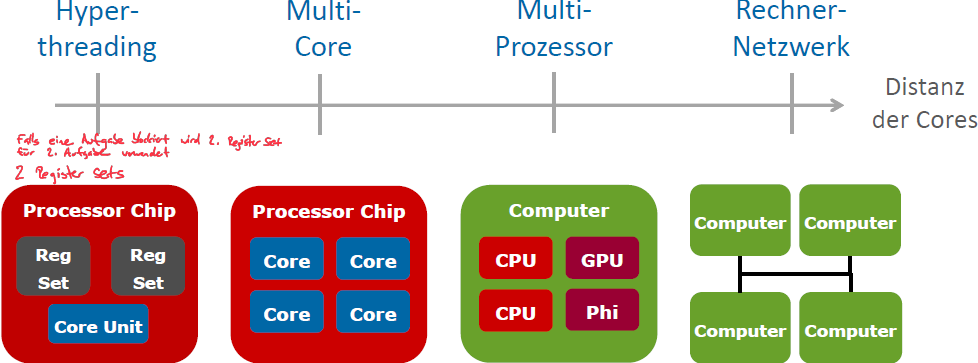
\includegraphics[width=\linewidth]{img/stufen.png}
\textbf{Parallelität:} Aufteilung in Teilabläufe, laufen gleichzeitig auf mehreren Prozessoren.
\textbf{Nebenläufigkeit:} Gleichzeitig oder verzahnt ausführbare Abläufe, greifen au gemeinsame Ressourcen zu.
\textbf{Prozess:} Parallel laufende Programm-Instanz im System. Eigener Adressraum.
\textbf{Thread:} Parallele Ablaufsequenz innerhalb eines Programms. Teilen gleichen Adressraum.

\subsection{Thread-Implementationen}
\textbf{User-Level Threads:} Im Prozess implementiert.
Keine echte Parallelität durch mehrere Prozessoren.
\textbf{Kernel-Level Threads:} Im Kernel implementiert (Multi-Core Ausnutzung).
Kontextwechsel vom Prozess per SW-Interrupt.
\textbf{Thread Scheduling:} Processor Sharing - \#Threads \textgreater \#Prozessoren.

\subsection{Prozessor Multiplexing}
\textbf{Verzahnte Ausführung:} Instruktionen von mehreren Threads in Teilsequenzen. Illusion der Parallelität.
\textbf{Kontextwechsel:} \textit{Synchron} (Freiwillige abgabe), Thread wechselt zu wait. \textit{Asynchron:} (gezwungene Abgabe) Begrenzte Laufzeit für Threads.

\subsection{Multi-Tasking:}
\textbf{Kooperativ:} Threads initiieren Kontextwechsel synchron (freiwillig). Scheduler kann Thread nicht unterbrechen.
\textbf{Preemtiv:} Scheduler kann Thread mit Timer-Interrupt asynchron unterbrechen (Time-Sliced-Scheduling)(\textit{Standart heute}).
\textbf{Thread Zustände:} Ready, Waiting, Running.

\subsection{Multi-Thread Programmierung}
\subsubsection{JVM Thread Modell}
Java ist ein Single Process System. 
JVM ist ein Prozess im Bsys.
\textbf{Main-Thread} wird beim Aufstarten der JVM anhand \textit{main()} Methode erzeugt.
JVM läuft, solange Threads laufen (Ausnahme Daemon Threads).
\begin{lstlisting}
var myThread = new Thread(() -> { /* ... */ });
myThread.start();
\end{lstlisting}
Thread wird erst bei \textit{start()} erzeugt. Führt \textit{run()}-Methode des Runnable Interface aus.
Thread endet beim Verlassen von \textit{run()}.\\
\textbf{Nicht-Determinismus:} Threads laufen ohne Vorkehrungen beliebig verzahnt oder parallel.
\subsubsection{Explizite Runnable-Implementation:}
\begin{lstlisting}
class SimpleLogic implements Runnable {
    @Override
    public void run() { /* ... */ }
}
var myThread = new Thread(new SimpleLogic()).start();
\end{lstlisting}

\subsubsection{Sub-Klasse von Thread}
\begin{lstlisting}
class SimpleThread extends Thread {
    @Override 
    public void run() { /* ... */ }
}
var myThread = new SimpleThread().start();
\end{lstlisting}

\subsubsection{Thread Join}
Warten auf Beendigung eines Threads. \textit{t2.join()} blockiert, solange t2 läuft.

\subsubsection{Thread Passivierung}
\textbf{Thraed.sleep(ms):} Laufender Thread geht in Wartezustand, dann ready.
\textbf{Thread.yield():} Gibt Prozesor frei, direkt ready.
        
\section{Monitor Synchronisation}
\subsection{Java Synchronized Methoden}
\begin{lstlisting}
synchronized void f() { /* ... */ } // Object Lock
static synchronized void g() { /* ... */ } // Class Lock
\end{lstlisting}

\subsection{Monitor}
Objekt mit internem gegenseitigem Ausschluss. Nur 1 Thread operiert im Monitor. Alle äusseren Methoden synchronized.
\textbf{Wait \& Signal Mechanismus:} Threads können im Monitor auf Bedingung warten und wartende aufwecken (signal).

\begin{lstlisting}
public synchronized void withdraw(int a) {
    while (amout > balance) { wait(); }
    balance -= a;
}
public synchronized void deposit(int a) {
    balance+= amount; notifyAll();
}
\end{lstlisting}
\textbf{notify():} Bei Uniform Waiters \& One-In-One-Out Bedingungen.
\textbf{notifyAll():} Bei mehreren Bedingungen / One-In-Multiple-Out. 
\textbf{Pauschales wait \& signal:} Wartende müssen selber schauen, ob sie ein Signal interessiert.
\textbf{Signal and Continue:} Signalisierender Thread behält Monitor nach notify. Aufgeweckter Thread muss um Monitor-Eintritt kämpfen.
        \section{Spezifische Synchronisationsprimitiven}
\subsection{Arten}
\textbf{Faire Semaphoren:} \textit{new Semaphore(N, true)}, FIFO Warteschlange, langsamer.

\begin{lstlisting}
private Semaphore upperL = new Semaphore(CAP, true);
private Semaphore lowerL = new Semaphore(0, true);
public void put(T item) throws InterruptedException {
    upperL.acquire();
    synchronized (queue) { queue.add(item); }
    lowerL.release();
}
public T get() throws InterruptedException {
    T item; lowerL.aquire();
    synchronized (queue) { item = queue.remove(); }
    upperL.release(); return item;
}
\end{lstlisting}
\textbf{Multi-Acquire/Release:} \textit{acquire(N)}.

\subsection{Lock \& Condition}
Monitor mit mehreren Wartelisten für verschiedene Bedingungen.
\textbf{Lock-Objekt:} Sperre für Eintritt in Monitor.
\textbf{Condition-Objekt:} Wait \& Signal für bestimmte Bedingung.

\begin{lstlisting}
private Lock monitor = new ReentrantLock(true); // fair
private Condition nonFull = monitor.newCondition();
private Condition nonEmpty = monitor.newCondition();
public void put(T item) throws InterruptedException {
    monitor.lock();
    try {
        while(queue.size() == Capacity) { nonFull.await(); }
        queue.add(item);
        nonEmpty.signal();
    } finally { monitor.unlock(); }
}
public T get() throws InterruptedException {
    monitor.lock();
    try {
        while(queue.size() == 0) { nonEmpty.await(); }
        T item = queue.remove();
        nonFull.signal();
        return item;
    } finally { monitor.unlock(); }
}
\end{lstlisting}

\subsection{Read-Write Locks}
Gegenseitiger Ausschluss ist unnötig streng für lesende Abschnitte.
Erlaube parallele Lese-Zugriffe.

\begin{lstlisting}
private Collection<String> names = new HashSet<>();
private ReadWriteLock rwLock = new ReentrantReadWriteLock();
public boolean exists(String pattern) { // Read-only accesses
    rwLock.readLock().lock();
    try {
        return names.steram().anyMatch(n -> n.matches(pattern));
    } finally { rwLock.readLock().unlock(); }
}
public void insert(String name) { // Write / Read accesses
    rwLock.writeLock().lock();
    try {
        names.add(name);
    } finally { rwLock.writeLock().unlock(); }
}
\end{lstlisting}

\subsection{Count Down Latch}
Synchronisationsprimitive mit Count Down Zähler.
Threads können warten, bis Zähler <= 0 wird.
\textbf{await():} warten bis Count Down 0 ist.
\textbf{countDown():} Zähler - 1.

\begin{lstlisting}
var ready = new CountDownLatch(N); // Warte auf N cars
var start = new CountDownLatch(1); // Einer gibt signal
// N Cars:
ready.countDown(); start.await();
// RaceControl:
ready.await(); start.countDown();
\end{lstlisting}

\subsection{Cyclic Barrier}
Treffpunkt für fixe Anzahl Threads. Anzahl treffender Threads muss vorgegeben sein.
Ist wiederverwendbar (mehrere Runden).

\begin{lstlisting}
var start = new CyclicBarrier(N); // Treffende Autos
// N Cars:
start.await(); // braucht kein Race Control mehr

var gameRound = new CyclicBarrier(N);
// N Players:
while(true) {
    gameRound.await(); // play concurrently with others
}

// Mit Austausch
Exchanger.exchange(something);
// Blockiert bis anderer Thread auch exchange() aufruft.
\end{lstlisting}
        \section{Gefahren der Nebenläufigkeit}
Neue Arten von Programmierfehler, die es bei single-Threading nicht gibt. 
Können sporadisch oder selten auftreten.
Sehr schwierig durch Tests zu finden.

\subsection{Race Condition}
Mehrere Threads greifen auf gemeinsame Ressourcen ohne genügend synchronisation zu.
Mögliche falsche Resultate oder falsches Verhalten.
Ursache oft ein Data Race, nicht immer.

\subsubsection{Data Race}
Unsynchronisierter Zugriff auf gleichen Speicher.
Selbe Variable oder Array Element (min. 1 schreibender Zugriff).

\subsubsection{Race Condition ohne Data Race}
Critical Sections nicht geschützt. 
Data Races mit Synchronisation eliminiert, aber nicht genügend grosse synchronisierte Blöcke.
\begin{lstlisting}
synchronized int getBalance() { return balance; }
synchronized void setBalance(int x) { balance = x; }
// Mehrere Threads, Kein Atomares Inc - Lost Update moeglich 
accout.setBalance(account.getBalance() + 100);
\end{lstlisting}

\subsubsection{Kombinationen}
\textbf{Alles Synchronisieren?} Hilft nichts. Race Condition trotzdem möglich. Weitere Nebenläufigkeitsfehler.
Synchronisationskosten sind relativ teuer.

\subsection{Synchronisation: Verzichtbare Fälle}
\textbf{Immutability (Unveränderlicheit):} Objekte mit nur lesendem Zugriff.
\textbf{Confinement (Einsperrung):} Objekt gehört nur einem Thread zu einer Zeit.

\subsubsection{Immutable Objects}
Instanzvariablen alle \textit{final}. Primitive Datentypen. Referenzen wiederum auf Immutable Objekte.
Methoden mit nur lesendem Zugriff. Konstruktor initialisiert Instanzvariablen.
Nach Konstruktor kann Objekt ohne Synchronisation von Threads verwendet werden.

\subsubsection{Confinement}
Struktur garantiert, dass auf ein Objekt nur durch einen Thread zur gleichen Zeit zugegriffen wird.
\textbf{Thread Confinement:} Objekt gehört nur einem Thread und wird nur von demjenigen verwendet.
\textbf{Object Confinement:} Objekt in anderem bereits synchronisierten Objekt eingekapselt.\\ 
\textbf{Kapselungsbrüche:} 1. Inneres Objekt ist aussen zugreifbar. 2. Rückgabe einer Referenz auf inneres Objekt.
3. Holder installiert selber Referenz ausserhalb. 4. Inneres Objekt gibt selber \textit{this} raus.


\subsection{Thread Safety}
Klassen / Methoden, die intern synchronisiert sind. Keine Race Conditions innerhalb dieses Codes.
Kritischer Abschnitt nur pro Methode erfüllt.
\textbf{Aber:} Kein kritischer Abschnitt über mehrere Methodenaufrufe. 
Andere Nebenläufigkeitsfehler möglich.

\subsubsection{Java Collections - Thread Safety}
Alte Java 1.0 Collections (Vector, Stack, Hashtable): \textbf{JA}. 
Moderne Collections (HashSet, TreeSet, ArrayList, etc.): \textbf{NEIN}.
Concurrent Collections (ConcurrentHashMap, etc.): \textbf{JA}.

\subsection{Verstecktes Multi-Threading}
\textbf{Finalizers:} Laufen über separaten Finalizer-Thread.
\textbf{Timers:} Handler durch separaten Thread ausgeführt (ausser GUI).
\textbf{Externe Libraries \& Frameworks:} z.B. Abarbeitung von Web-Service Aufrufen.

\subsection{Deadlock}
Beide Threads sperren sich gegenseitig aus:
\begin{lstlisting}
syncrhonized(listA) { // Thread 1
    syncrhonized(listB) {
        listB.addAll(listA);
    }
}
synchronized(listB) { // Thread 2
    synchronized(listA) {
        listA.addAll(listB);
    }
}
\end{lstlisting}

\subsubsection{Spezialfall: Livelocks}
Threads haben sich gegenseitig permanent blockiert. Führen aber noch Warteinstruktionen aus.
Verbrauchen CPU während Deadlock.
\begin{lstlisting}
// Thread 1
b = false; while (!a) { } b = true;
// Thread 2
a = false; while (!b) { } a = true;
\end{lstlisting}

\subsubsection{Deadlock Erkennung}
\textit{Deadlock = Zyklus im Betriebsmittelgraph}\\ 
\textbf{Deadlock Voraussetzungen:} Geschachtelte Locks, Zyklische Warteabhänigkeiten

\subsubsection{Deadlock Vermeidung}
\textbf{Lineare Sperrordnung} der Ressourcen einführen. 
Nur geschachtelt in aufsteigender Reihenfolge sperren. 
Eliminiert zyklische Warteabhänigkeiten.\\ 
\textbf{Grobgranulare Locks} wählen.
Wenn lineare Sperrordnung nicht möglich/sinvoll ist.
Sperre gesamte Bank bei Kontenzugriff.
Eliminiert Schachtelung von Locks.

\subsection{Starvation}
Ein Thread kriegt nie die Chance, auf eine Ressource zuzugreifen, obwohl sie immer wieder frei wird.
Andere Threads überholen andauernd. Liveness/Fairness Problem.
\begin{lstlisting}
do { // Starvation moeglich 
    success = account.widthdraw(100);
} while (!success);
\end{lstlisting}

\subsubsection{Vermeidung}
Faire Synchronisationskonstrukte (bei Semaphore, Lock \& Condition, ReadwriteLock möglich).
Java Monitor hat ein Fairness Problem (Starvation anfällig).

\subsection{Parallelität Korrektheitskriterien}
\textbf{Safety:} Keine Race Conditions, Keine Deadlocks.
\textbf{Liveness:} Keine Starvation.

    \end{multicols*}
\end{document}

























